\flushbottom








%%============================================================================
%%============================================================================
\chapter{Laplace's Equation}















%%=============================================================================
\section{Introduction}


Laplace's equation in $n$ dimensions is
\[
\Delta u = 0
\]
where
\[
\Delta = \frac{\partial^2}{\partial x_1^2} + \cdots + \frac{\partial^2}{\partial x_n^2}.
\]


The inhomogeneous analog is called \textbf{Poisson's Equation}.
\[
- \Delta u = f(\mathbf{x})
\]

CONTINUE





%%=============================================================================

\section{Fundamental Solution}



The fundamental solution of Poisson's equation in $\mathbb{R}^n$ satisfies
\[
- \Delta G = \delta(\mathbf{x} - \mathbf{\xi}).
%% CONTINUE is the LaTeX right?
\]


%%----------------------------------------------------------------------------
\subsection{Two Dimensional Space}


If $n = 2$ then the fundamental solution satisfies
\[
- \left(\frac{\partial^2}{\partial x^2} + \frac{\partial^2}{\partial y^2}\right) G = \delta(x - \xi) \delta(y - \psi).
\]
Since the product of delta functions, $\delta(x - \xi) \delta(y - \psi)$ is 
circularly symmetric about the point $(\xi,\psi)$, we look for a solution in 
the form $u(x,y) = v(r)$ where $r = \sqrt((x - \xi)^2 + (y - \psi)^2)$.





CONTINUE















\raggedbottom
%%=============================================================================
\exercises{
\pagebreak
\flushbottom
\section{Exercises}









\begin{Exercise}
Is the solution of the following Dirichlet problem unique?
\begin{gather*}
  u_{x x} + u_{y y} = q(x,y), \quad -\infty < x < \infty, \quad y > 0
  \\
  u(x,0) = f(x)
\end{gather*}
\end{Exercise}






\begin{Exercise}
Is the solution of the following Dirichlet problem unique?
\begin{gather*}
  u_{x x} + u_{y y} = q(x,y), \quad -\infty < x < \infty, \quad y > 0
  \\
  u(x,0) = f(x), \quad u\ \mathrm{bounded as}\ x^2 + y^2 \to \infty
\end{gather*}
\end{Exercise}






\begin{Exercise}
Not all combinations of boundary conditions/initial
conditions lead to so called well-posed problems. Essentially, a well posed
problem is one where the solutions depend continuously on the boundary data. 
Otherwise it is considered ``ill posed''. 

Consider Laplace's equation on the unit-square
\[ 
u_{x x} + u_{y y} = 0,
\] 
with $u(0,y) = u(1,y) = 0$ and $u(x,0) = 0$, $u_y(x,0) = \epsilon \sin(n \pi x)$.
\begin{enumerate}
\item 
  Show that even as $\epsilon \to 0$, you can find $n$ so that
  the solution can attain any finite value for any $y > 0$. Use this to then
  show that this problem is ill posed. 
\item 
  Contrast this with the case where  $u(0,y) = u(1,y) = 0$ and $u(x,0) = 0$, 
  $u(x,1) = \epsilon \sin(n \pi x)$. Is this well posed? 
\end{enumerate}
\end{Exercise}








\begin{Exercise}
Use the fundamental solutions for the Laplace equation
\[
\nabla^2 G = \delta(\mathbf{x}-\boldsymbol{\xi})
\]
in three dimensions
\[ 
G(\mathbf{x}|\boldsymbol{\xi}) = - \frac{1}{4 \pi |\mathbf{x} - \boldsymbol{\xi}|}
\]
to derive the mean value theorem for harmonic functions
\[ 
u(\mathbf{p}) = \frac{1}{4 \pi R^2} \int_{\partial S_R} u(\boldsymbol{\xi})
\,\dd A_{\boldsymbol{\xi}},
\]
that relates the value of any harmonic function $u(\mathbf{x})$ at the point
$\mathbf{x} = \mathbf{p}$ to the average of its value on the boundary of 
the sphere of radius $R$ with center at $\mathbf{p}$, ($\partial S_R$). 
\end{Exercise}








\begin{Exercise}
Use the fundamental solutions for the modified Helmholz equation
\[
\nabla^2 u - \lambda u = \delta(\mathbf{x} - \boldsymbol{\xi})
\]
in three dimensions
\[ 
u_\pm(\mathbf{x}|\boldsymbol{\xi})= \frac{-1}{4 \pi |\mathbf{x} - \boldsymbol{\xi}|} 
\e^{\pm \sqrt{\lambda} |\mathbf{x} - \boldsymbol{\xi}|},
\]
to derive a ``generalized'' mean value theorem:
\[ 
\frac{ \sinh \left( \sqrt{\lambda} R \right) }{ \sqrt{\lambda} R } u(\mathbf{p}) 
= \frac{1}{4 \pi R^2} \int_{\partial S} u(\mathbf{x}) \,\dd A
\]
that relates the value of any solution $u(\mathbf{x})$ at a point
$P$ to the average of its value on the sphere of radius $R$ ($\partial S$) 
with center at P. 
\end{Exercise}






\begin{Exercise}
Consider the uniqueness of solutions of $\nabla^2 u(\mathbf{x}) = 0$ in a
two dimensional region $R$ with boundary curve $C$ and a boundary condition
$\mathbf{n} \cdot \nabla u(\mathbf{x}) = -a (\mathbf{x})u(\mathbf{x})$ on $C$. State
a non-trivial condition on the function $a(\mathbf{x})$ on $C$ for which 
solutions are unique, and justify your answer. 
\end{Exercise}







%% On semi-infinite cylinder.
\begin{Exercise}
Solve Laplace's equation on the surface of a semi-infinite cylinder
of unit radius, $0 < \theta < 2 \pi$, $z > 0$, where the solution, 
$u(\theta, z)$ is prescribed at $z = 0$: $u(\theta, 0) = f(\theta)$.  
\end{Exercise}







%% On a rectangle with four inhomogeneous boundaries.
\begin{Exercise}
Solve Laplace's equation in a rectangle.
\begin{gather*}
  w_{x x} + w_{y y} = 0, \quad 0 < x < a, \quad 0 < y < b, 
  \\
  w(0, y) = f_1(y), \quad w(a, y) = f_2(y), 
  \\
  w_y(x, 0) = g_1(x), \quad w(x, b) = g_2(x)
\end{gather*}
Proceed by considering $w = u + v$ where $u$ and $v$ are harmonic and 
satisfy
\begin{gather*}
  u(0, y) = u(a, y) = 0, \quad u_y(x, 0) = g_1(x), \quad u(x, b) = g_2(x), 
  \\
  v(0, y) = f_1(y), \quad v(a, y) = f_2(y), \quad v_y(x, 0) = v(x, b) = 0.
\end{gather*}
\end{Exercise}








\raggedbottom
}
%%=============================================================================
\hints{
\pagebreak
\flushbottom
\section{Hints}






\begin{Hint}
%% CONTINUE
\end{Hint}






\begin{Hint}
%% CONTINUE
\end{Hint}







\begin{Hint}
%% CONTINUE
\end{Hint}






\begin{Hint}
%% CONTINUE
\end{Hint}





\begin{Hint}
%% CONTINUE
\end{Hint}








\begin{Hint}
%% CONTINUE
\end{Hint}











%% On semi-infinite cylinder.
\begin{Hint}
%% CONTINUE
\end{Hint}













%% On a rectangle with four inhomogeneous boundaries.
\begin{Hint}
%% CONTINUE
\end{Hint}












\raggedbottom
}
%%=============================================================================
\solutions{
\pagebreak
\flushbottom
\section{Solutions}










\begin{Solution}
Let $u$ and $v$ both be solutions of the Dirichlet problem.
Let $w$ be the difference of these solutions.  $w$ satisfies the problem
\begin{gather*}
  w_{x x} + w_{y y} = 0, \quad -\infty < x < \infty, \quad y > 0
  \\
  w(x,0) = 0.
\end{gather*}
Since $w = c y$ is a solution. We conclude that the solution of the 
Dirichlet problem is not unique.
\end{Solution}










\begin{Solution}
Let $u$ and $v$ both be solutions of the Dirichlet problem.
Let $w$ be the difference of these solutions.  $w$ satisfies the problem
\begin{gather*}
  w_{x x} + w_{y y} = 0, \quad -\infty < x < \infty, \quad y > 0
  \\
  w(x,0) = 0, \quad w\ \mathrm{bounded as}\ x^2 + y^2 \to \infty.
\end{gather*}
We solve this problem with a Fourier transform in $x$.
\begin{gather*}
  - \omega^2 \hat{w} + \hat{w}_{y y} = 0, \quad \hat{w}(\omega,0) = 0, \quad 
  \hat{w}\ \mathrm{bounded as}\ y \to \infty
  \\
  \hat{w} = \begin{cases}
    c_1 \cosh{\omega y} + c_2 \sinh(\omega y), &\omega \neq 0 \\
    c_1 + c_2 y, &\omega = 0
  \end{cases}
  \\
  \hat{w} = 0
  \\
  w = 0
\end{gather*}
Since $u - v = 0$, we conclude that the solution of the Dirichlet problem
is unique.
\end{Solution}








\begin{Solution}
\begin{enumerate}
\item 
  We seek a solution of the form $u(x,y) = \sin(n \pi x) Y(y)$.  This form 
  satisfies the boundary conditions at $x = 0,1$.
  \begin{gather*}
    u_{x x} + u_{y y} = 0
    \\
    -(n \pi)^2 Y + Y'' = 0, \quad Y(0) = 0
    \\
    Y = c \sinh(n \pi y)
  \end{gather*}
  Now we apply the inhomogeneous boundary condition.
  \begin{gather*}
    u_y(x,0) = \epsilon \sin(n \pi x) = c n \pi \sin(n \pi x)
    \\
    u(x,y) = \frac{\epsilon}{n \pi} \sin(n \pi x) \sinh(n \pi y)
  \end{gather*}
  For $\epsilon = 0$ the solution is $u = 0$.  Now consider any $\epsilon > 0$.  For any
  $y > 0$ and any finite value $M$, we can choose a value of $n$ such that 
  the solution along $y = 0$ takes on all values in the range $[-M \ldots M]$.
  We merely choose a value of $n$ such that
  \[
  \frac{\sinh(n \pi y)}{n \pi} \geq \frac{M}{\epsilon}.
  \]
  Since the solution does not depend continuously on boundary data, this 
  problem is ill posed.
\item 
  We seek a solution of the form $u(x,y) = c \sin(n \pi x) \sinh(n \pi y)$.  
  This form satisfies the differential equation and the boundary conditions 
  at $x = 0,1$ and at $y = 0$.
  We apply the inhomogeneous boundary condition at $y = 1$.
  \begin{gather*}
    u(x,1) = \epsilon \sin(n \pi x) = c \sin(n \pi x) \sinh(n \pi)
    \\
    u(x,y) = \epsilon \sin(n \pi x) \frac{\sinh(n \pi y)}{\sinh(n \pi)}
  \end{gather*}
  For $\epsilon = 0$ the solution is $u = 0$.  Now consider any $\epsilon > 0$.  Note that
  $|u| \leq \epsilon$ for $(x,y) \in [0 \ldots 1] \times [0 \ldots 1]$.  The solution depends 
  continuously on the given boundary data.  This problem is well posed.
\end{enumerate}
\end{Solution}








\begin{Solution}
The Green function problem for a sphere of radius $R$ centered at the point
$\boldsymbol{\xi}$ is
\begin{equation}
  \label{eqn DG=d, G=0}
  \Delta G = \delta(\mathbf{x} - \boldsymbol{\xi}), \quad
  G \big|_{|\mathbf{x} - \boldsymbol{\xi}| = R} = 0.
\end{equation}
We will solve Laplace's equation, $\Delta u = 0$, where the value of $u$ is
known on the boundary of the sphere of radius $R$ in terms of this 
Green function.

First we solve for $u(\mathbf{x})$ in terms of the Green function.
\[
\int_S (u \Delta G - G \Delta u) \,\dd \boldsymbol{\xi}
= \int_S u \delta(\mathbf{x} - \boldsymbol{\xi}) \,\dd \boldsymbol{\xi}
= u(\mathbf{x})
\]
\begin{align*}
  \int_S (u \Delta G - G \Delta u) \,\dd \boldsymbol{\xi}
  &= \int_{\partial S} \left( u \frac{\partial G}{\partial n} - G \frac{\partial u}{\partial n} \right) \,\dd A_{\boldsymbol{\xi}}
  \\
  &= \int_{\partial S} u \frac{\partial G}{\partial n} \,\dd A_{\boldsymbol{\xi}}
\end{align*}
\[
u(\mathbf{x}) = \int_{\partial S} u \frac{\partial G}{\partial n} \,\dd A_{\boldsymbol{\xi}}
\]
We are interested in the value of $u$ at the center of the sphere.  
Let $\rho = |\mathbf{p} - \boldsymbol{\xi}|$
\[
u(\mathbf{p}) = \int_{\partial S} u(\boldsymbol{\xi}) 
\frac{\partial G}{\partial \rho}(\mathbf{p}|\boldsymbol{\xi}) \,\dd A_{\boldsymbol{\xi}}
\]

We do not need to compute the general solution of 
Equation~\ref{eqn DG=d, G=0}.  We only need the Green function at the 
point $\mathbf{x} = \mathbf{p}$.  We know that the general solution of the
equation $\Delta G = \delta(\mathbf{x} - \boldsymbol{\xi})$ is 
\[
G(\mathbf{x}|\boldsymbol{\xi}) = - \frac{1}{4 \pi |\mathbf{x} - \boldsymbol{\xi}|}
+ v(\mathbf{x}),
\]
where $v(\mathbf{x})$ is an arbitrary harmonic function.
The Green function at the point $\mathbf{x} = \mathbf{p}$ is 
\[
G(\mathbf{p}|\boldsymbol{\xi}) = - \frac{1}{4 \pi |\mathbf{p} - \boldsymbol{\xi}|}
+ \mathrm{const}.
\]
We add the constraint that the Green function vanishes at $\rho = R$.  
This determines the constant.
\begin{gather*}
  G(\mathbf{p}|\boldsymbol{\xi}) = - \frac{1}{4 \pi |\mathbf{p} - \boldsymbol{\xi}|}
  + \frac{1}{4 \pi R}
  \\
  G(\mathbf{p}|\boldsymbol{\xi}) = - \frac{1}{4 \pi \rho}
  + \frac{1}{4 \pi R}
  \\
  G_\rho(\mathbf{p}|\boldsymbol{\xi}) = \frac{1}{4 \pi \rho^2}
  \\
\end{gather*}

Now we are prepared to write $u(\mathbf{p})$ in terms of the Green function.
\begin{gather*}
  u(\mathbf{p}) = \int_{\partial S} u(\boldsymbol{\xi}) \frac{1}{4 \pi \rho^2} \,\dd A_{\boldsymbol{\xi}}
  \\
  u(\mathbf{p}) = \frac{1}{4 \pi R^2} \int_{\partial S} u(\boldsymbol{\xi}) \,\dd A_{\boldsymbol{\xi}}
\end{gather*}
This is the Mean Value Theorem for harmonic functions.
\end{Solution}








\begin{Solution}
The Green function problem for a sphere of radius $R$ centered at the point
$\boldsymbol{\xi}$ is
\begin{equation}
\label{eqn DG-lG=d, G=0}
\Delta G - \lambda G = \delta(\mathbf{x} - \boldsymbol{\xi}), \quad
G \big|_{|\mathbf{x} - \boldsymbol{\xi}| = R} = 0.
\end{equation}
We will solve the modified Helmholtz equation,
\[
\Delta u - \lambda u = 0,
\]
where the value of $u$ is known on the boundary of the sphere of 
radius $R$ in terms of this Green function.

in terms of this Green function.

Let $L[u] = \Delta u - \lambda u$.
\[
\int_S (u L[G] - G L[u]) \,\dd \boldsymbol{\xi}
= \int_S u \delta(\mathbf{x} - \boldsymbol{\xi}) \,\dd \boldsymbol{\xi}
= u(\mathbf{x})
\]
\begin{align*}
  \int_S (u L[G] - G L[u]) \,\dd \boldsymbol{\xi}
  &= \int_S (u \Delta G - G \Delta u) \,\dd \boldsymbol{\xi}
  \\
  &= \int_{\partial S} \left( u \frac{\partial G}{\partial n} - G \frac{\partial u}{\partial n} \right) \,\dd A_{\boldsymbol{\xi}}
  \\
  &= \int_{\partial S} u \frac{\partial G}{\partial n} \,\dd A_{\boldsymbol{\xi}}
\end{align*}
\[
u(\mathbf{x}) = \int_{\partial S} u \frac{\partial G}{\partial n} \,\dd A_{\boldsymbol{\xi}}
\]
We are interested in the value of $u$ at the center of the sphere.  
Let $\rho = |\mathbf{p} - \boldsymbol{\xi}|$
\[
u(\mathbf{p}) = \int_{\partial S} u(\boldsymbol{\xi}) 
\frac{\partial G}{\partial \rho}(\mathbf{p}|\boldsymbol{\xi}) \,\dd A_{\boldsymbol{\xi}}
\]

We do not need to compute the general solution of 
Equation~\ref{eqn DG-lG=d, G=0}.  We only need the Green function at the 
point $\mathbf{x} = \mathbf{p}$.  We know that the Green function there is a 
linear combination of the fundamental solutions,
\[
G(\mathbf{p}|\boldsymbol{\xi}) = c_1 \frac{-1}{4 \pi |\mathbf{p} - \boldsymbol{\xi}|} 
\e^{\sqrt{\lambda} |\mathbf{p} - \boldsymbol{\xi}|}
+ c_2 \frac{-1}{4 \pi |\mathbf{p} - \boldsymbol{\xi}|} 
\e^{-\sqrt{\lambda} |\mathbf{p} - \boldsymbol{\xi}|},
\]
such that $c_1 + c_2 = 1$.  The Green function is symmetric with respect to 
$\mathbf{x}$ and $\boldsymbol{\xi}$.  We add the constraint that the 
Green function vanishes at $\rho = R$.  This gives us two equations for 
$c_1$ and $c_2$.
\begin{gather*}
  c_1 + c_2 = 1, \quad 
  - \frac{c_1}{4 \pi R} \e^{\sqrt{\lambda} R} - \frac{c_2}{4 \pi R} \e^{-\sqrt{\lambda} R} = 0
  \\
  c_1 = - \frac{1}{ \e^{2 \sqrt{\lambda} R} - 1 }, \quad
  c_2 = \frac{ \e^{ 2 \sqrt{\lambda} R } }{ \e^{2 \sqrt{\lambda} R} - 1 }
  \\
  G(\mathbf{p}|\boldsymbol{\xi}) 
  = \frac{ \sinh \left( \sqrt{\lambda} (\rho - R) \right) }
  { 4 \pi \rho \sinh \left( \sqrt{\lambda} R \right) }
  \\
  G_\rho(\mathbf{p}|\boldsymbol{\xi}) 
  = \frac{ \sqrt{\lambda} \cosh \left( \sqrt{\lambda} (\rho - R) \right) }
  { 4 \pi \rho \sinh \left( \sqrt{\lambda} R \right) }
  - \frac{ \sinh \left( \sqrt{\lambda} (\rho - R) \right) }
  { 4 \pi \rho^2 \sinh \left( \sqrt{\lambda} R \right) }
  \\
  G_\rho(\mathbf{p}|\boldsymbol{\xi}) \big|_{|\boldsymbol{\xi}| = R}
  = \frac{ \sqrt{\lambda} }{ 4 \pi R \sinh \left( \sqrt{\lambda} R \right) }
\end{gather*}
Now we are prepared to write $u(\mathbf{p})$ in terms of the Green function.
\begin{gather*}
  u(\mathbf{p}) = \int_{\partial S} u(\boldsymbol{\xi}) 
  \frac{ \sqrt{\lambda} }{ 4 \pi \rho \sinh \left( \sqrt{\lambda} R \right) } \,\dd A_{\boldsymbol{\xi}}
  \\
  u(\mathbf{p}) = \int_{\partial S} u(\mathbf{x}) 
  \frac{ \sqrt{\lambda} }{ 4 \pi R \sinh \left( \sqrt{\lambda} R \right) } \,\dd A
\end{gather*}
Rearranging this formula gives us the generalized mean value theorem.
\[
\frac{ \sinh \left( \sqrt{\lambda} R \right) }{ \sqrt{\lambda} R } u(\mathbf{p}) 
= \frac{1}{4 \pi R^2} \int_{\partial S} u(\mathbf{x}) \,\dd A
\]
\end{Solution}








\begin{Solution}
First we think of this problem in terms of the the equilibrium solution of the 
heat equation.  The boundary condition expresses Newton's law of cooling.
Where $a = 0$, the boundary is insulated.  Where $a > 0$, the rate of heat
loss is proportional to the temperature.  The case $a < 0$ is non-physical
and we do not consider this scenario further.
We know that if the boundary is entirely insulated, $a = 0$, then the 
equilibrium temperature is a constant that depends on the initial 
temperature distribution.  Thus for $a = 0$ the solution of Laplace's equation
is not unique.  If there is any point on the boundary where $a$ is positive
then eventually, all of the heat will flow out of the domain.  The equilibrium
temperature is zero, and the solution of Laplace's equation is unique, 
$u = 0$.  Therefore the solution of Laplace's equation is unique if 
$a$ is continuous, non-negative and not identically zero.



Now we prove our assertion.  First note that if we substitute 
$\mathbf{f} = v \nabla u$ in the divergence theorem,
\[
\int_R \nabla \cdot \mathbf{f} \,\dd \mathbf{x} 
= \int_{\partial R} \mathbf{f} \cdot \mathbf{n} \,\dd s,
\]
we obtain the identity,
\begin{equation}
  \label{eqn int vu+vu = int vun}
  \int_R ( v \Delta u + \nabla v \nabla u ) \,\dd \mathbf{x} 
  = \int_{\partial R} v \frac{\partial u}{\partial n} \,\dd s.
\end{equation}
Let $u$ be a solution of Laplace's equation subject to the Robin boundary
condition with our restrictions on $a$.  We take $v = u$ in
Equation~\ref{eqn int vu+vu = int vun}.
\[
  \int_R (\nabla u)^2 \,\dd \mathbf{x} 
  = \int_C u \frac{\partial u}{\partial n} \,\dd s
  = - \int_C a u^2 \,\dd s
\]
Since the first integral is non-negative and the last is non-positive, 
the integrals vanish.  This implies that $\nabla u = 0$.  $u$ is a constant.
In order to satisfy the boundary condition where $a$ is non-zero, $u$ must
be zero.  Thus the unique solution in this scenario is $u = 0$.
\end{Solution}










%% On semi-infinite cylinder.
\begin{Solution}
The mathematical statement of the problem is
\begin{gather*}
  \Delta u \equiv u_{\theta \theta} + u_{z z} = 0, \quad 0 < \theta < 2 \pi, \quad z > 0, 
  \\
  u(\theta, 0) = f(\theta).
\end{gather*}
We have the implicit boundary conditions,
\[
u(0, z) = u(2 \pi, z), \quad u_\theta(0, z) = u_\theta(0, z)
\]
and the boundedness condition,
\[
u(\theta, +\infty)\ \mathrm{bounded}.
\]
We expand the solution in a Fourier series. (This ensures that the boundary 
conditions at $\theta = 0, 2\pi$ are satisfied.)
\[
u(\theta, z) = \sum_{n = -\infty}^\infty u_n(z) \e^{\imath n \theta}
\]
We substitute the series into the partial differential equation to obtain
ordinary differential equations for the $u_n$.
\[
-n^2 u_n(z) + u_n''(z) = 0
\]
The general solutions of this equation are
\[
u_n(z) = \begin{cases}
  c_1 + c_2 z, &\mathrm{for}\ n = 0, \\
  c_1 \e^{n z} + c_2 \e^{-n z} &\mathrm{for}\ n \neq 0.
\end{cases}
\]
The bounded solutions are
\[
u_n(z) = \begin{cases}
  c \e^{-n z}, &\mathrm{for}\ n > 0, \\
  c,      &\mathrm{for}\ n = 0, \\
  c \e^{n z}, &\mathrm{for}\ n < 0,
\end{cases}
= c \e^{-|n| z}.
\]
We substitute the series into the initial condition at $z = 0$ to determine
the multiplicative constants.
\begin{gather*}
  u(\theta, 0) = \sum_{n = -\infty}^\infty u_n(0) \e^{\imath n \theta} = f(\theta) 
  \\
  u_n(0) = \frac{1}{2 \pi} \int_0^{2 \pi} f(\theta) \e^{-\imath n \theta} \,\dd \theta \equiv f_n
\end{gather*}
Thus the solution is
\[
\boxed{
  u(\theta, z) = \sum_{n = -\infty}^\infty f_n \e^{\imath n \theta} \e^{-|n| z}.
}
\]
Note that
\[
u(\theta, z) \to f_0 = \frac{1}{2 \pi} \int_0^{2 \pi} f(\theta)\,\dd \theta
\]
as $z \to +\infty$.
\end{Solution}













%% On a rectangle with four inhomogeneous boundaries.
\begin{Solution}
The decomposition of the problem is shown in Figure~\ref{lap_rect}.
\begin{figure}[h!]
\begin{center}
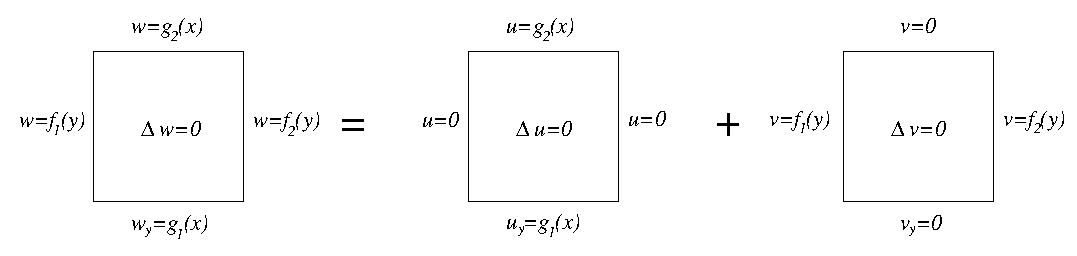
\includegraphics[width=\textwidth]{pde/laplace/lap_rect}
\end{center}
\caption{Decomposition of the problem.}
\label{lap_rect}
\end{figure}


First we solve the problem for $u$.
\begin{gather*}
u_{x x} + u_{y y} = 0, \quad 0 < x < a, \quad 0 < y < b, \\
u(0, y) = u(a, y) = 0, \\
u_y(x, 0) = g_1(x), \quad u(x, b) = g_2(x)
\end{gather*}
We substitute the separation of variables $u(x, y) = X(x) Y(y)$ into 
Laplace's equation.
\[
\frac{X''}{X} = - \frac{Y''}{Y} = - \lambda^2
\]
We have the eigenvalue problem,
\[
X'' = - \lambda^2 X, \quad X(0) = X(a) = 0,
\]
which has the solutions,
\[
\lambda_n = \frac{n \pi}{a}, \quad X_n = \sin \left( \frac{n \pi x}{a} \right),
        \quad n \in \mathbb{N}.
\]
The equation for $Y(y)$ becomes,
\[
Y_n'' = \left( \frac{n \pi}{a} \right)^2 Y_n,
\]
which has the solutions,
\[
\left\{
\e^{n \pi y / a}, \e^{-n \pi y / a}
\right\}
\quad \mathrm{or} \quad
\left\{
\cosh\left( \frac{n \pi y}{a} \right), \sinh\left( \frac{n \pi y}{a} \right)
\right\}.
\]
It will be convenient to choose solutions that satisfy the conditions,
$Y(b) = 0$ and $Y'(0) = 0$, respectively.
\[
\left\{
\sinh \left( \frac{n \pi (b - y)}{a} \right),
\cosh\left( \frac{n \pi y}{a} \right)
\right\}
\]
The solution for $u(x, y)$ has the form,
\[
u(x, y) = \sum_{n = 1}^\infty \sin \left( \frac{n \pi x}{a} \right)
        \left( \alpha_n \sinh \left( \frac{n \pi (b - y)}{a} \right)
        + \beta_n \cosh\left( \frac{n \pi y}{a} \right) \right).
\]
We determine the coefficients from the inhomogeneous boundary conditions.
(Here we see how our choice of solutions for $Y(y)$ is convenient.)
\begin{gather*}
u_y(x, 0) = \sum_{n = 1}^\infty - \frac{n \pi}{a} \alpha_n 
        \sin \left( \frac{n \pi x}{a} \right)
        \cosh \left( \frac{n \pi b}{a} \right) = g_1(x) \\
\alpha_n = - \frac{a}{n \pi} \sech \left( \frac{n \pi b}{a} \right)
        \frac{2}{a} \int_0^a g_1(x) \sin \left( \frac{n \pi x}{a}\right)\,\dd x\\
u(x, y) = \sum_{n = 1}^\infty \beta_n \sin \left( \frac{n \pi x}{a} \right)
        \cosh\left( \frac{n \pi y}{a} \right) \\
\beta_n = \sech \left( \frac{n \pi b}{a} \right)
        \frac{2}{a} \int_0^a g_2(x) \sin \left( \frac{n \pi x}{a} \right)\,\dd x
\end{gather*}


Now we solve the problem for $v$.
\begin{gather*}
v_{x x} + v_{y y} = 0, \quad 0 < x < a, \quad 0 < y < b, \\
v(0, y) = f_1(y), \quad v(a, y) = f_2(y), \\
v_y(x, 0) = 0, \quad v(x, b) = 0
\end{gather*}
We substitute the separation of variables $u(x, y) = X(x) Y(y)$ into 
Laplace's equation.
\[
\frac{X''}{X} = - \frac{Y''}{Y} = \lambda^2
\]
We have the eigenvalue problem,
\[
Y'' = - \lambda^2 Y, \quad Y'(0) = Y(b) = 0,
\]
which has the solutions,
\[
\lambda_n = \frac{(2 n - 1)\pi}{2 b}, \quad 
        Y_n = \cos \left( \frac{(2 n - 1) \pi y}{2 b} \right),
        \quad n \in \mathbb{N}.
\]
The equation for $X(y)$ becomes,
\[
X_n'' = \left( \frac{(2 n - 1) \pi}{2 b} \right)^2 X_n.
\]
We choose solutions that satisfy the conditions, $X(a) = 0$ and $X(0) = 0$, 
respectively.
\[
\left\{
\sinh \left( \frac{(2 n - 1) \pi (a - x)}{2 b} \right),
\sinh \left( \frac{(2 n - 1) \pi x}{2 b} \right)
\right\}
\]
The solution for $v(x, y)$ has the form,
\[
v(x, y) = \sum_{n = 1}^\infty \cos \left( \frac{(2 n - 1) \pi y}{2 b} \right)
        \left( \gamma_n \sinh \left( \frac{(2 n - 1) \pi (a - x)}{2 b} \right)
        + \delta_n \sinh \left( \frac{(2 n - 1) \pi x}{2 b} \right) \right).
\]
We determine the coefficients from the inhomogeneous boundary conditions.
\begin{gather*}
v(0, y) = \sum_{n = 1}^\infty \gamma_n \cos \left( \frac{(2 n - 1) \pi y}{2 b} \right)
        \sinh \left( \frac{(2 n - 1) \pi a}{2 b} \right) = f_1(y) \\
\gamma_n = \csch \left( \frac{(2 n - 1) \pi a}{2 b} \right) \frac{2}{b}
        \int_0^b f_1(y) \cos \left( \frac{(2 n - 1) \pi y}{2 b} \right)\,\dd y\\
v(a, y) = \sum_{n = 1}^\infty \delta_n \cos \left( \frac{(2 n - 1) \pi y}{2 b} \right)
        \sinh \left( \frac{(2 n - 1) \pi a}{2 b} \right) = f_2(y) \\
\delta_n = \csch \left( \frac{(2 n - 1) \pi a}{2 b} \right) \frac{2}{b}
        \int_0^b f_2(y) \cos \left( \frac{(2 n - 1) \pi y}{2 b} \right)\,\dd y
\end{gather*}
With $u$ and $v$ determined, the solution of the original problem is 
$w = u + v$.
\end{Solution}













\raggedbottom
}
